\documentclass{article}

\RequirePackage{epsfig}

\RequirePackage{graphics}

\ExecuteOptions{dvipsone}

\title{Language Driven Software Engineering}

\author{Tony Clark}

\begin{document}

\maketitle

\section{Introduction}

Traditional methods of system development, such as {\em top-down decomposition}, arose at a time
when computer applications tended to be written in a single language and for execution on a single 
machine. At that time, applications centered around business logic -- issues such as databases,
human interfaces and distribution architectures were second class citizens.

Over the last decade, computer applications have become much more sophisticated and the technology
used to implement them has become diverse. It is no longer the case that an application consists
of a single large block of code with some simple interfaces. Applications tend to be distributed,
where the responsibility for processing information is decentralised and spread much more evenly
between the application components. Furthermore, implementation technologies vary from component
to component and there is a corresponding increase in the complexity of the {\em glue} code
necessary to allow components work together.

Traditional development methods do not work well in this new environment. A significant contribution
to this failure is that traditional methods do not take into account the possibility of
multiple components each working in a different way. The essential {\em behaviour} of components
and the corresponding {\em behaviour} of an integration framework is as much a part of the
system design as the essential business logic.

To be successful in this new distributed and diverse world of system development, methods must
support a behavioural view of the system that captures the essential features of execution
but which do not commit to technology issues too early. Methods must identify the key aspects of
execution and use technologies that express these aspects succinctly. Methods must provide
a means of introducing implementation detail when a developer is ready to commit; it must
be possible to introduce this detail step-by-step. 

Recent proposals for development methods are starting to address these issues. The Object
Management Group (OMG) has proposed Model Driven Architecture (MDA). The MDA method advocates
modelling the essential features of an application as a Platform Independent Model (PIM). A
PIM is then translated to a Platform Specific Model (PSM) where implementation detail is
introduced. The idea is that, as technology changes, the same PIM can be re-translated 
without re-defining the essential application features. 

A number of proposals have been made for {\em domain specific languages} (DSLs) where
languages are defined to suit the application at hand. The languages are either defined
in the deployed application environment or are the source of a translation to the
deployed application environment.

UML 2.0 has introduced the notion of a {\em component} that captures the structure and
interface of a system component. Connectors are used to combine components to produce
applications. Connectors describe the type of implementation technology that will be
required to realize the communication between components.

MDA, DSLs and UML 2.0 components address problems of modern system development; however they
do not clearly identify the key aspects of the problems that they claim to address. For 
example, MDA does not make clear the distinction between a PIM and a PSM or what would
constitute a valid translation from one to the other. Components have been proposed as
good Software Engineering practice for many years; however UML 2.0 components miss an 
essential ingredient -- the behaviour of the architecture used to host the various components.

DSLs have traditionally been proposed by researchers from abstract languages such as
functional programming.Often, researchers have embedded a DSL in an existing prototyping
language where efficiency considerations are not a primary concern. It is unclear how a 
commercial application is produced. 

This note proposes a view of systems development that addresses the features of modern
systems. The view includes features of MDA and components, but extends them by requiring
that system {\em behaviour} is explicitly addressed. System development is viewed as
{\em language definition}. Abstract languages ({\em i.e.} idealized languages) are used 
to capture the essential features of application components {\em including its behaviour}. 
Abstract component architectures are used to capture the essential characteristics
of inter-component communication. Concrete languages ({\em i.e.} languages that exist) and
concrete architectures are the target of MDA-style transformations. 

\section{Components}

An application consists of a collection of components and a component architecture. 
Components define logically self-contained units of an application, for example
a planning component, a billing component or a user interface component. This section
discusses how components are represented in LDSE. 

\begin{figure}
\begin{center}
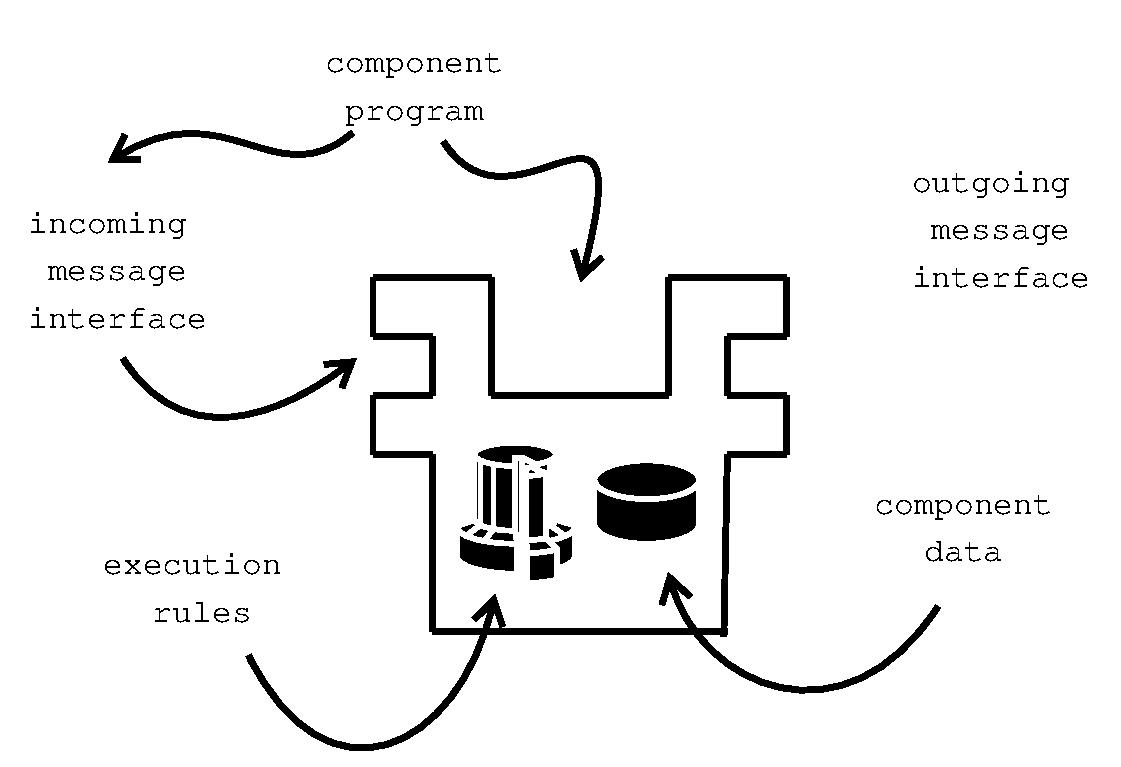
\includegraphics[scale=0.5]{Component.eps}
\end{center}
\caption{A Component}
\label{Component}
\end{figure}

Figure \ref{Component} shows the essential features of a component. It is an independent
execution engine, with its own state, running a given program processing inputs from its
{\em in} interface and producing outputs on its {\em out} interface. 

A component is associated with a language definition consisting of the following:

\begin{itemize}

\item A definition of the execution rules for running the component. This may take
any number of forms, for example: a prototype program written in a concrete language;
a collection of transition rules; an interpreter; or a real programming language such
as Java or Ada. It is very desirable for the execution rule definition to be executable.

\item A definition of the data (or {\em semantic data items}) processed by the
component. This can take the form of simple abstract data types such as sets and
trees or it can take the form of concrete data types from a particular programming
language such as Java arrays or Ada strings.

\item A definition of the language syntax. The component will execute programs written
in this language. The component's execution engine runs a supplied program in the context
of the data managed by the component. The program syntax definition could be a concrete
language such as Java or Ada. On the other hand the language could be an abstract domain
specific language that is defined to capture the essential features of the components's
domain.

\item The component's interfaces. A component processes messages supplied from its
environment and produces messages to the environment. A component is embedded in an
architecture that provides its environment.

\end{itemize}
An important feature of LDSE is that each component is defined with respect to
its own language. Domain specific languages can be used along-side concrete languages when
defining an application. It is important when defining a DSL that the language definition
is complete ({\em i.e.} contains the definition of syntax and semantics) since in 
order to deploy a system design, the complete DSL will need to be transformed to a concrete
language.

It could be argued that an approach that requires the developer to specify a complete
language for each component in an application is unworkable in terms of the amount
of work that is necessary. However, this is exactly what expert system developers do
when formulating an initial definition of a system. Each component is expressed (informally
at least) using an idealized execution engine; the developer then uses experience of
systems implementation to map the idealized component to a concrete component. Experience
has shown the developer how to apply transformations to the component so that
the idealized executions are faithfully represented in terms of a concrete implementation.
Component executions are completely described in terms of the component's data; its 
execution rules; its program structure and its input/output messages.

The approach does not require fresh languages to be developed for each new component.
LDSE relies on suitable languages being used for each component. If an existing language
exists that is close to what is required then it can readily be modified or used as-is.
Typically, DSLs are fairly simple languages that capture the essential features of an
application. Concrete languages are embraced by the approach, but component languages
would not need to be built for these since they exist already. 

LDSE is essentially about realising that in order to develop component-based software; 
we need to address the issues of component-languages and relationships between the component 
languages.

\section{Architectures and Systems}

System architectures manage communications between components. Typical architectures
are peer-to-peer and server-client. LDSE views architectures as multi-component language
engines. Architectures run programs that control the execution engine for the architecture.
The execution engine controls a number of components as part of its state.

A system is constructed by placing components into an architecture. An architecture is reponsible 
for managing the communication between the components. An architecture is a {\em component
combinator} that takes components and returns a new component. The new architecture
component can then be viewed as an independent unit that manages a collection of sub-components
in order to supply a given interface.

\begin{figure}
\begin{center}
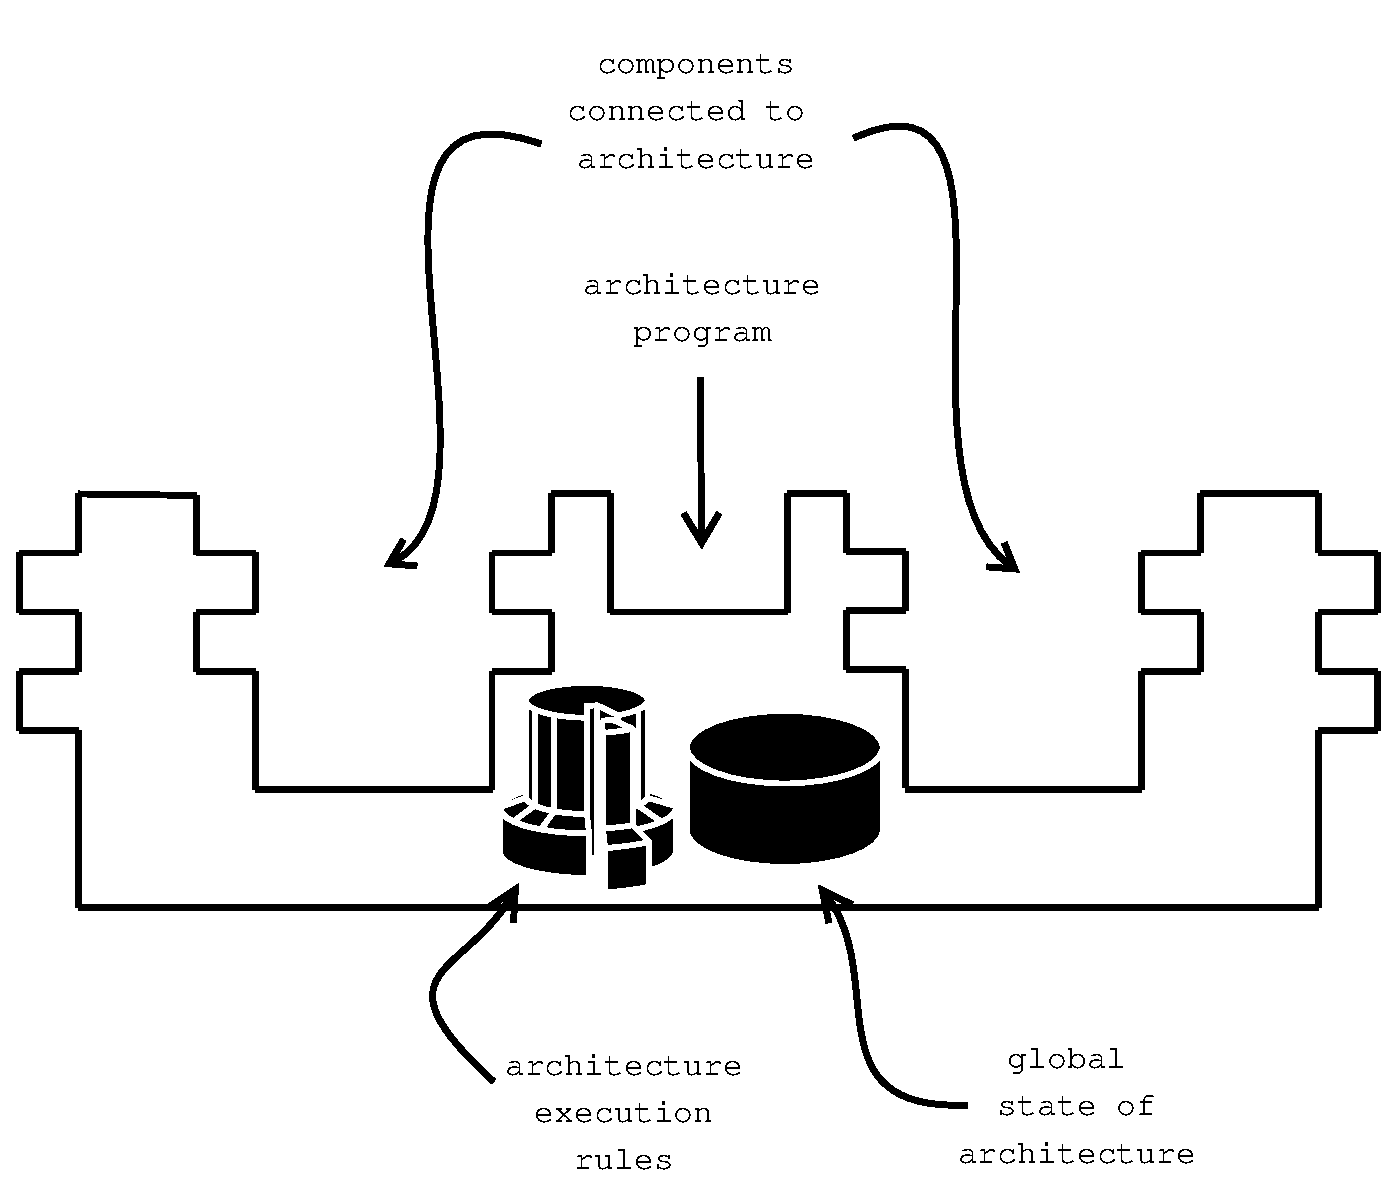
\includegraphics[scale=0.5]{Architecture.eps}
\end{center}
\caption{An Architecture}
\label{Architecture}
\end{figure}

A 2-component architecture is shown in figure \ref{Architecture}. Like a component, an architecture
provides an interface; has state; expects a program and has execution rules. In addition,
an architecture allows components to be plugged in - the components become part of the
architecture state and are controlled by the architecture's execution engine. In general an
architecture may have any number of components.

Once an architecture is fully defined, it becomes a component that can be combined with
other components and added to other architectures. A system can therefore be defined as an
onion-like combination of components and architectures. Alternatively, we can view a
system as a single component and then zoom in to ever increasing levels of detail showing 
communicating components.

Since we are describing both an abstract view of systems engineering in addition to a concrete 
method it is possible to use the view of architectures and components decompose a system in
different ways, each reflecting the aspects and partitioning of the system that is appropriate
to the view we wish to take.

\section{Patterns}

Component and architecture patterns are incomplete definitions (or equivalently
parametric definitions). For example, the client-server architecture patterns is a
parametric architecture with two arguments: the server component and the client
component. A peer-to-peer architecture pattern has n argument components for the
communicating peers.

\section{Mappings}

MDA and DSLs take the view that a system should be developed by defining models and
languages that are specific to the application domain. Analysing this view of the system
and then deplying a concrete system by transforming the abstract components to concrete
components.

LDSE also takes this view although it goes further by identifying the key components 
of the transformation and therefore the essential features of the checks that must take place
in order to ensure that the transformation is valid.

\begin{figure}
\begin{center}
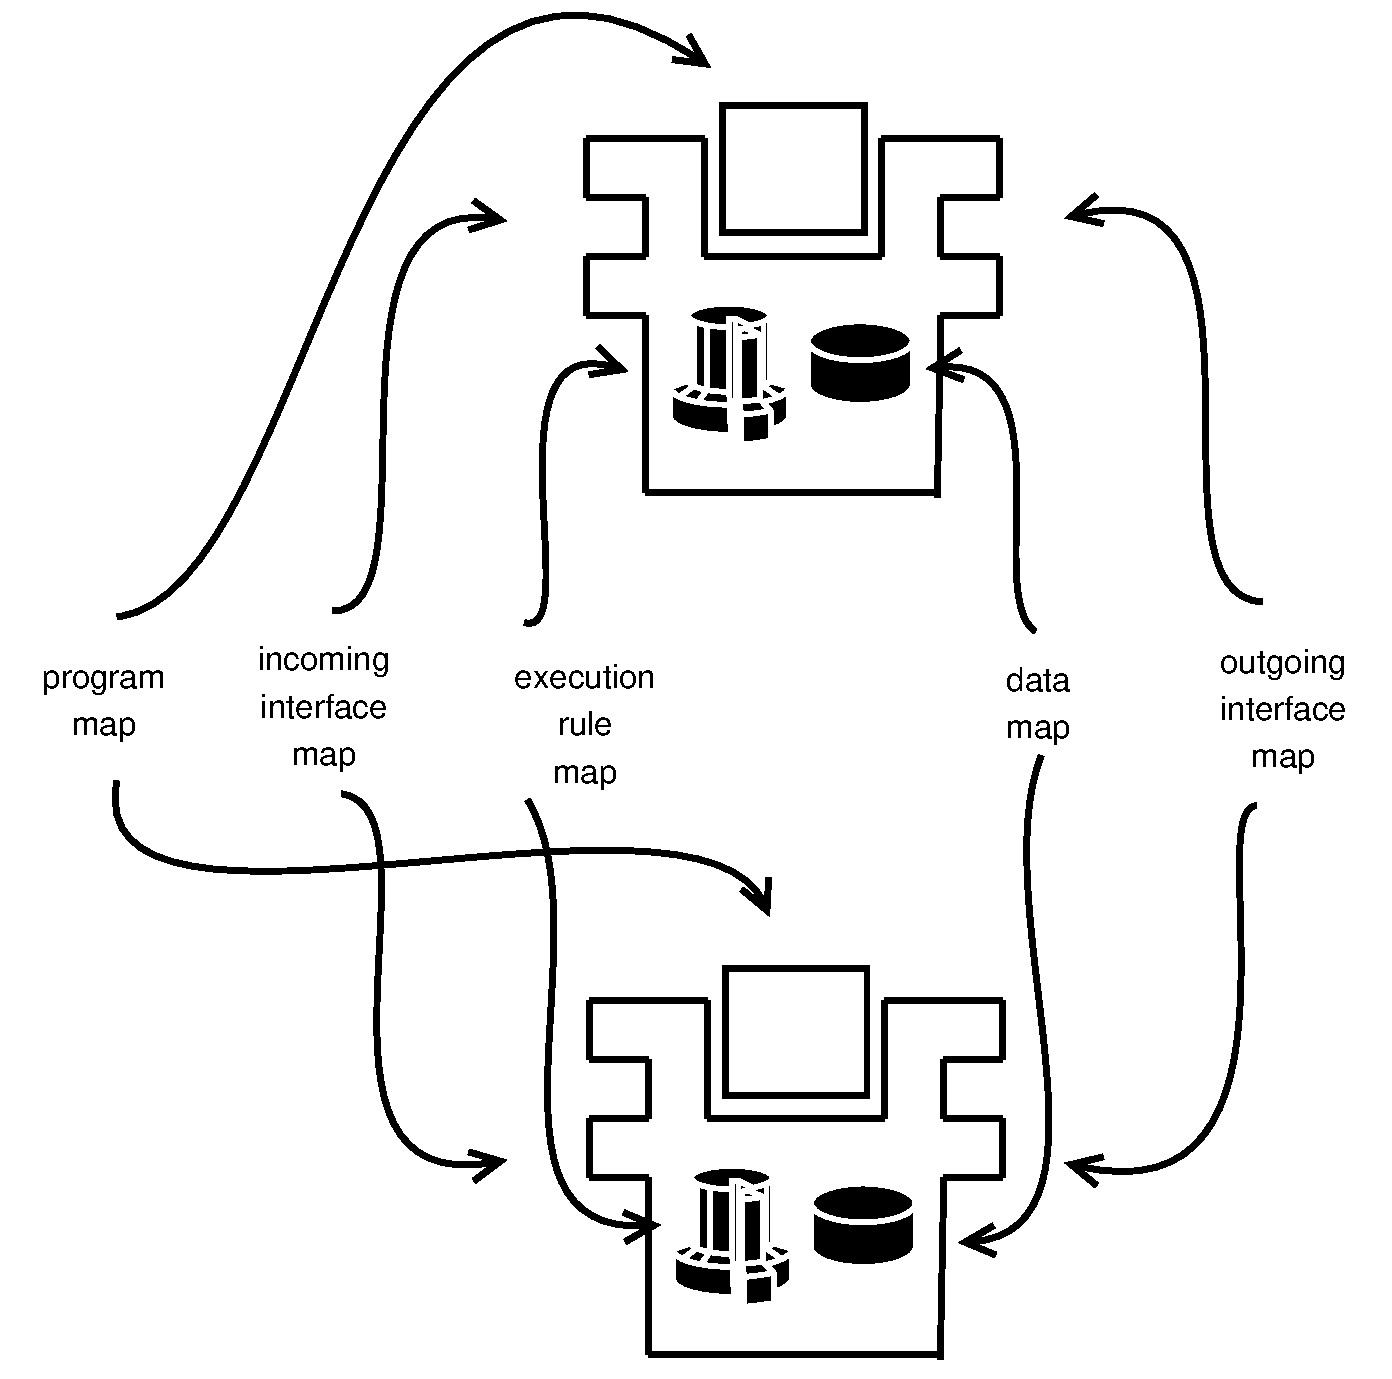
\includegraphics[scale=0.5]{ComponentMapping.eps}
\end{center}
\caption{Component Mapping}
\label{ComponentMapping}
\end{figure}

Figure \ref{ComponentMapping} shows the elements of a component mapping. In general two
components are mapped by associating the individual elements. The mapping may be partial,
total, determinstic or non-deterministic. The most general form of mapping is a partial
statement of key features in each component and how they are realised in the other
component. For example, each type of data element from one component can be described
in terms of the data types of the other component. In this, most general, form there need
not be any requirement that all of either component can be supported by the other component.

In practice, it is usually the case that one of the components is a more abstract ({\em i.e.}
simpler) description of the other component. In this case we want to arrive at a situation 
where all of the abstract component can be shown to be embedded in the more concrete
component. Therefore we want the mapping to be total; however, it need not be deterministic.
A total and deterministic mapping can be performed mechanically providing it is finite for
any finite input.

The essential elements of a component mapping are:

\begin{itemize}

\item A mapping between data formats. This shows how to represent data from one component 
in the data types available to the other component. An example of this (in a PIM to
PSM style mapping) is where sets in the abstract component are implemented as Java vectors.

\item A mapping between execution rules. This mapping shows how to take the execution rules
from one component and represent them as executions in the other component. For example,
sets could be manipulated using set selection and set element operators in an abstract
PIM whereas in Java we need to use a collection of Vector methods to realize each set
operation.

\item A mapping between the interfaces of the components. This shows how to translate 
events and messages occurring in the interface of one component into the equivalent events
and messages in the other component.

\item A mapping between programs. This shows how to turn programs from one component
into programs in the other component. For example we might use an OCL based language
or an action language in a PIM. The expressions and actions may be transformed to Java in
a PSM.

\end{itemize}
Note that to construct a total mapping for a completely described pair of components is
a large undertaking. However, in general we can choose to undertake LDSE in a number of ways.
LDSE may inform our view of system design in which case the rules of mapping construction are 
guidelines that should be part of a QA process. Given that LSDS components have programs,
we are likely to have a number of reusable component available to use with examples of
pre-constructed mappings. In addition, many component languages are likely to be variations
on a theme; existing components and mappings can easily be modified for the job at hand.

Note also that PIMs, by their very nature, are likely to be an order of magnitude (at least)
simpler than the corresponding PSM. Therefore, if we are practising MDA then the mapping
from PIM to PSM acts like a compiler for the PIM language. Given that the PIM language
is an order smaller that of the PSM, then the mapping is equivalent to constructing a
simple prototype translator for a language that is 10 -- 100 times simpler than the PSM
language. With tool support this is not an unreasonable undertaking.

\section{System Development}

A number of approaches to system development have been proposed including top-down and 
bottom up methods, formal methods, iterative refinement. LDSE is intended to support
all of these approaches. For example, a top-down approach defines the system as a single
component with a complete interface. Development steps map the single component to a 
collection of decomposed components and introduces an architecture to manage the interactions.

Bottom-up methods involve defining all the individual concrete components for aspects
of the application and then gradually combining these components into larger components
using architectures.

\section{Example}

Consider the development of a standard enterprise information system involving a web
based interface that allows customers to browse a catalogue, select items, and
place orders. The system prvides middelware that encodes the business logic controlling
the catalogue and the order system. Finally, the system uses a database to store the
current stock, catalogue elements and customer orders.

An initial step is to define a single component that provides the complete interface.
The language for this component is event based; it handles all user interface requests 
and manages the system data as a single global data structure.

After constructing an executable component as above, it is noticed that the interface
aspect of the component language can be separated out; as can the database aspect of the
language. Three components are proposed:

\begin{itemize}

\item A component for the interface. The language is based on input form description and
uses a state transition machine to define how a user session progresses from form to
form. The input interface accepts user events. The output interface produces messages
to perform system operations.

\item A component for the business logic. The language is anything that is suitable for processing
abstract data -- such as OCL. The data for this component is records and collections of data.
The input interface processes messages requesting system functionality. The output 
interface produces messages that request data and perform form updates.

\item A database component. The language is SQL or OCL with actions. The data is sets of records.

\end{itemize}
Given three components it is necessary to define an architecture that explains how
they interact. The architecture  simply passes messages around.

Given a complete description of the components and architecture necessary to define the 
system we can then map each individually to concrete implementations. This can be done in
a variety of ways. Here is an example:

\begin{itemize}

\item The interface component is translated to a component supporting HTML and JavaScript.

\item The business logic component is transformed into a component supporting
session and entity beans where the PIM language
is translated to Java.

\item The database component is translated into a component supporting a concrete RDBS.

\item The architecture is translated into J2EE where the interpretive mechanism of the source
architecture is translated to a suitable implementation in Java.

\end{itemize}

\end{document}